\documentclass{../vespers-booklet}
\usepackage{multicol}

\begin{document}

% TODO: Update the title for the specific feast
\chapter*{Second Vespers of the Solemnity of our Holy Father Benedict}

\begin{center}
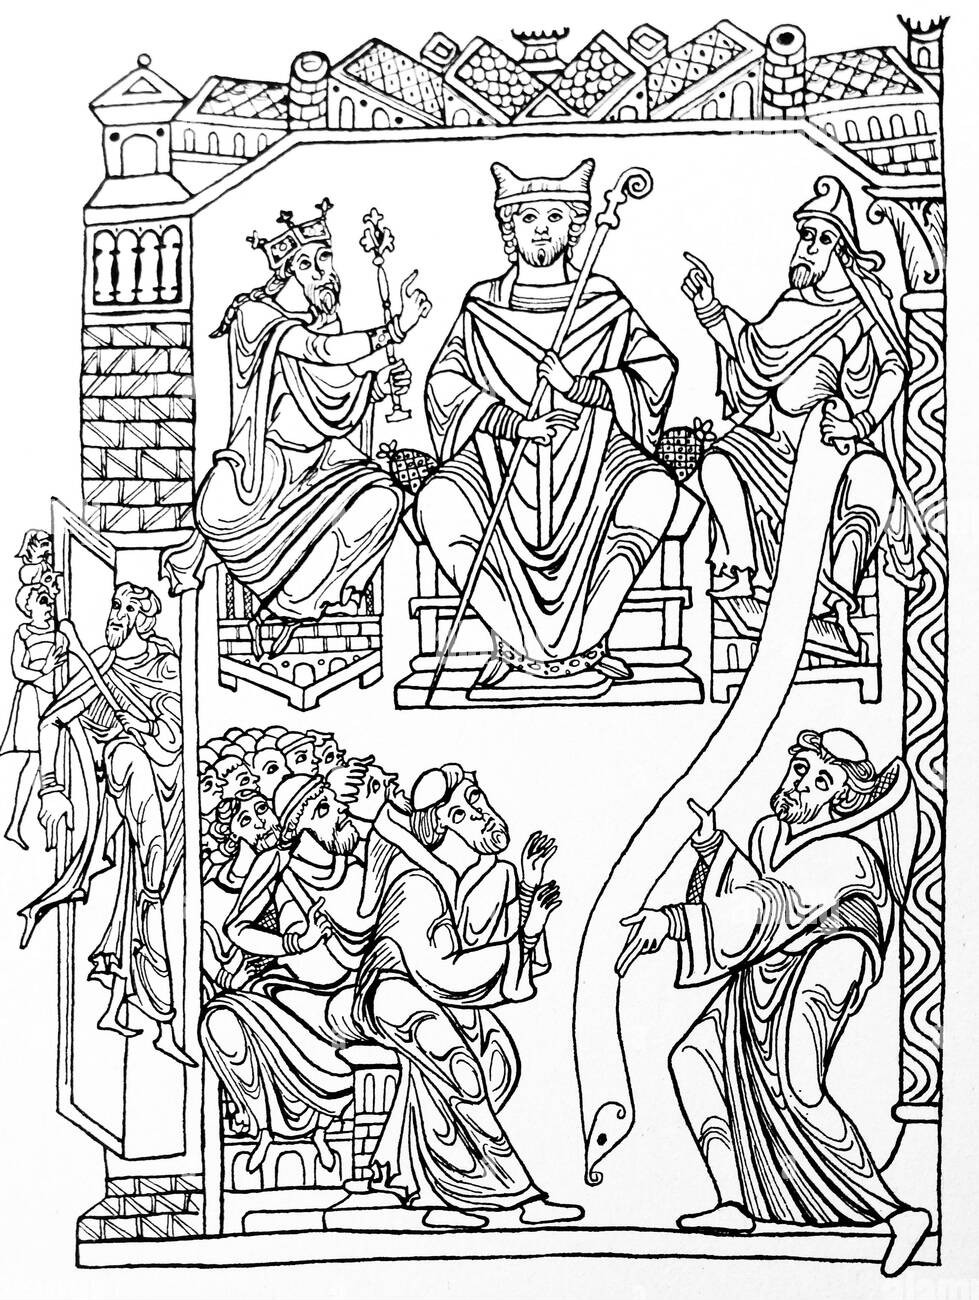
\includegraphics[width=0.7\linewidth]{benedict_rule_reading_c}
\end{center}

\vfill\newpage

%\section*{Beginning of the Office}

\begin{rubricbox}

{\color{red}When the Officiant kneels, all \textbf{kneel} and pray silently.
Then, when the Officiant stands, all \textbf{stand} and say silently one \textit{Pater noster} (Our Father) and \textit{Ave Maria} (Hail Mary).
Then all make the sign of the cross with the Officiant as he intones:}

\end{rubricbox}

% TODO: Make sure that the tone of the deus adjutorium matches the season primarily and the solemnity of the feast secondarily
 \gresetinitiallines{1}
\gregorioscore{../common/deus-in-adjutorium-solemn}

\textit{
O God, come to my assistance.
{\color{red}\Vbar.}~O Lord, make haste to help me.
Glory be to the Father, and to the Son, and to the Holy Spirit,
as it was in the beginning, is now, and ever shall be, world without end. Amen.
Praise to Thee, O Lord, King of endless glory.}

%TODO: Add that the correct psalms, and verify that their tones, and their associated pointed text are correct

\section*{Psalm 109}

\textit{\textnormal{Ant. 1.} The man of God, Benedict, made the sign of the Cross; and the glass containing the deadly drink was broken into pieces, as if a stone had been hurled against it.
 \textnormal{Ps.} The Lord said to my Lord...}
 
 \begin{rubricbox}

{\color{red} All remain standing throughout the first antiphon.
After the psalm is intoned by the Cantor, all \textbf{sit} at the asterisk.}

\end{rubricbox}

\gresetinitiallines{1}
\gregorioscore{ps109-antiphon}

\gresetinitiallines{0}
\gregorioscore{ps109-intonation}

\begin{latinenglishsection}

\latinenglish{
	2. Donec ponam inimícos \textbf{tu}os,~* scabéllum pedum \textit{tu}\textbf{ó}rum.

3. Virgam virtútis tuæ emíttet Dóminus ex \textbf{Si}on:~* domináre in médio inimicórum \textit{tu}\textbf{ó}rum.

4. Tecum princípium in die virtútis tuæ in splendóribus sanc\textbf{tó}rum:~* ex útero ante lucíferum gé\textit{nu}\textbf{i} te.

5. Jurávit Dóminus, et non p{\oe}nitébit \textbf{e}um:~* Tu es sacérdos in ætérnum secúndum órdinem \textit{Mel}\textbf{chí}sedech.

6. Dóminus a dextris \textbf{tu}is,~* confrégit in die iræ su\textit{æ} \textbf{re}ges.

7. Judicábit in natiónibus, implébit ru\textbf{í}nas:~*\\ conquassábit cápita in terra \textit{mul}\textbf{tó}rum.

8. De torrénte in via \textbf{bi}bet:~* proptérea exaltá\textit{bit} \textbf{ca}put.

9. {\color{red}\textit{(bow)}} Glória Patri, et \textbf{Fí}lio,~* et Spirítu\textit{i} \textbf{Sanc}to.

10. {\color{red}\textit{(rise)}} Sicut erat in princípio, et nunc, et \textbf{sem}per,~* et in s\'{\ae}cula sæculó\textit{rum}. \textbf{A}men.
 %%
}{
	% 1. The Lord said to my Lord: Sit thou at my right hand:

2. Until I make thy enemies thy footstool.
 
3. The Lord will send forth the sceptre of thy power out of Sion: rule thou in the midst of thy enemies.
 
4. With thee is the principality in the day of thy strength: in the brightness of the saints:
 from the womb before the day star I begot thee.
 
5. The Lord hath sworn, and he will not repent: Thou art a priest for ever according to the order of Melchisedech.
 
6. The Lord at thy right hand hath broken kings in the day of his wrath.

7. He shall judge among nations, he shall fill ruins: he shall crush the heads in the land of the many.

8. He shall drink of the torrent in the way: therefore shall he lift up the head. 

Glory be. %%
}

\end{latinenglishsection}

\begin{rubricbox}

{\color{red}The antiphon is repeated: Vir Dei Benedictus\textit{\dots}} %%

\end{rubricbox}

\gresetinitiallines{1}
\gregorioscore{ps109-antiphon}

%%

\section*{Psalm 110}

\textit{\textnormal{Ant. 2.} When he had finished his prayer, he set up three stones to mark the spot, and almighty God supplied water on the rocky heights.
\textnormal{Ps.} I will praise thee, O Lord, with my whole heart...}

\begin{rubricbox}

{\color{red} The remaining psalms are said in the same manner as the first.}

\end{rubricbox}

\gresetinitiallines{1}
\gregorioscore{ps110-antiphon}

\gresetinitiallines{0}
\gregorioscore{ps110-intonation}

\begin{latinenglishsection}

\latinenglish{
	2. Magna ópera \textbf{Dó}mini:~*
	exquisíta in omnes volun\textit{tá}\textit{tes} \textbf{e}jus.

3. Conféssio et magnificéntia opus \textbf{e}jus:~*
	et justítia ejus manet in s\'{\ae}\textit{cu}\-\textit{lum} \textbf{s\'{\ae}}culi.

4. Memóriam fecit mirabílium suórum,~{\color{red}\GreDagger}\
	miséricors et miserátor \textbf{Dó}\-minus:~*
	escam dedit ti\textit{mén}\textit{ti}\textbf{bus} se.

5. Memor erit in s\'{\ae}culum testaménti \textbf{su}i:~*
	virtútem óperum suórum annuntiábit pó\textit{pu}\textit{lo} \textbf{su}o:

6. Ut det illis hereditátem \textbf{gén}ti\-um:~*
	ópera mánuum ejus véritas, \textit{et} \textit{ju}\textbf{dí}\-cium.

7. Fidélia ómnia mandáta ejus:~{\color{red}\GreDagger}\
	confirmáta in s\'{\ae}culum \textbf{s\'{\ae}}culi,~*
	facta in veritáte et \textit{æ}\textit{qui}\textbf{tá}te.

8. Redemptiónem misit pópulo \textbf{su}o:~*
	mandávit in ætérnum\\ testa\textit{mén}\textit{tum} \textbf{su}um.

9. Sanctum, et terríbile nomen \textbf{e}jus:~*
	inítium sapiéntiæ \textit{ti}\textit{mor} \textbf{Dó}\-mini.

10. Intelléctus bonus ómnibus faciéntibus \textbf{e}um:~*
	laudátio ejus manet in s\'{\ae}\textit{cu}\textit{lum} \textbf{s\'{\ae}}culi.

{\color{red}\textit{(bow)}} Glória Patri, et \textbf{Fí}lio,~*
	et Spirí\textit{tu}\textit{i} \textbf{Sanc}to.

{\color{red}\textit{(rise)}} Sicut erat in princípio, et nunc, et \textbf{sem}per,~*
	et in s\'{\ae}cula sæcu\textit{ló}\textit{rum}. \textbf{A}men.
}{
	 1. I will praise thee, O Lord, with my whole heart; in the council of the just: and in the congregation.
 
 2. Great are the works of the Lord: sought out according to all his wills.
 
 3. His work is praise and magnificence: and his justice continueth for ever and ever.
 
 4.  He hath made a remembrance of his wonderful works, being a merciful and gracious Lord: he hath given food to them that fear him. 	
 
 5. He will be mindful for ever of his covenant: he will shew forth to his people the power of his works.
 
 6. That he may give them the inheritance of the Gentiles: the works of his hands are truth and judgment.
 
 7. All his commandments are faithful: confirmed for ever and ever, made in truth and equity.
 
 8. He hath sent redemption to his people: he hath commanded his covenant for ever.
 
 9. Holy and terrible is his name: the fear of the Lord is the beginning of wisdom.
 
 10. A good understanding to all that do it: his praise continueth for ever and ever. 
}

\end{latinenglishsection}

%\begin{rubricbox}
%
%{\color{red}The antiphon is repeated: Completa oratione\textit{\dots}} %%
%
%\end{rubricbox}

\gresetinitiallines{1}
\gregorioscore{ps110-antiphon}

%%

\section*{Psalm 111}

\textit{\textnormal{Ant. 3.} After the glorious Confessor of the Lord said a prayer, he gave a blessing; and the stone upon which the ancient enemy had been sitting was raised immediately.
\textnormal{Ps.} Blessed is the man that feareth the Lord...}

\gresetinitiallines{1}
\gregorioscore{ps111-antiphon}

\gresetinitiallines{0}
\gregorioscore{ps111-intonation}

\begin{latinenglishsection}

\latinenglish{
	2. Potens in terra erit \textbf{se}men \textbf{e}jus:~* generátio rectórum be\textit{ne}\textit{di}\textbf{cé}tur.

3. Glória, et divítiæ in \textbf{do}mo \textbf{e}jus:~* et justítia ejus manet in s\'{\ae}\textit{cu}\textit{lum} \textbf{s\'{\ae}}culi.

4. Exórtum est in ténebris \textbf{lu}men \textbf{rec}tis:~* miséricors, et miserá\textit{tor}, \textit{et} \textbf{jus}tus.

5. Jucúndus homo qui miserétur et cómmodat,~{\color{red}\GreDagger} dispónet sermónes suos \textbf{in} ju\textbf{dí}\textbf{ci}o:~* quia in ætérnum non \textit{com}\textit{mo}\textbf{vé}bitur.

6. In memória ætérna \textbf{e}rit \textbf{jus}tus:~* ab auditióne mala \textit{non} \textit{ti}\textbf{mé}bit.

7. Parátum cor ejus speráre in Dómino,~{\color{red}\GreDagger} confirmátum \textbf{est} cor \textbf{e}jus:~* non commovébitur donec despíciat ini\textit{mí}\textit{cos} \textbf{su}os.

8. Dispérsit, dedit paupéribus:~{\color{red}\GreDagger} justítia ejus manet in \textbf{s\'{\ae}}culum \textbf{s\'{\ae}}\textbf{cu}li,~* cornu ejus exaltábi\textit{tur} \textit{in} \textbf{gló}ria.

9. Peccátor vidébit, et irascétur,~{\color{red}\GreDagger} déntibus suis fremet \textbf{et} ta\textbf{bé}scet:~* desidérium peccató\textit{rum} \textit{per}\textbf{í}bit.

10. {\color{red}\textit{(bow)}} Glória \textbf{Pa}tri, et \textbf{Fí}\textbf{li}o,~* et Spirí\textit{tu}\textit{i} \textbf{Sanc}to.

11. {\color{red}\textit{(rise)}} Sicut erat in princípio, et \textbf{nunc}, et \textbf{sem}per,~* et in s\'{\ae}cula sæcu\textit{ló}\textit{rum}. \textbf{A}men.
}{
	1. Blessed is the man that feareth the Lord: he shall delight exceedingly in his commandments.

2. His seed shall be mighty upon earth: the generation of the righteous shall be blessed.

3. Glory and wealth shall be in his house: and his justice remaineth for ever and ever.

4. To the righteous a light is risen up in darkness: he is merciful, and compassionate and just.

5. Acceptable is the man that sheweth mercy and lendeth: he shall order his words with judgment:
because he shall not be moved for ever.

6. The just shall be in everlasting remembrance: he shall not fear the evil hearing.

7. His heart is ready to hope in the Lord: his heart is strengthened, he shall not be moved until he look over his enemies.

8. He hath distributed, he hath given to the poor: his justice remaineth for ever and ever: his horn shall be exalted in glory.

9. The wicked shall see, and shall be angry, he shall gnash with his teeth and pine away: the desire of the wicked shall perish. 
}

\end{latinenglishsection}

%\begin{rubricbox}
%
%{\color{red}The antiphon is repeated: Gloriosus Confessor Domini\textit{\dots}} %%
%
%\end{rubricbox}

\gresetinitiallines{1}
\gregorioscore{ps111-antiphon}

%%

\vfill\pagebreak

\section*{Psalm 112}

\textit{\textnormal{Ant. 4.} When Placidus was carried out of the water, he saw above his head the robe of the Abbot, who was rescuing him from the waves.
\textnormal{Ps.} Praise the Lord, ye children...}

\gresetinitiallines{1}
\gregorioscore{ps112-antiphon}

\gresetinitiallines{0}
\gregorioscore{ps112-intonation}

\begin{latinenglishsection}

\latinenglish{
	 2.  Sit nomen Dómini \textbf{be}ne\-\textbf{díc}tum,~*
	ex hoc nunc, et \textbf{us}que in \textbf{s\'{\ae}}culum.

 3. A solis ortu usque \textbf{ad} oc\textbf{cá}sum,~*
	laudábile \textbf{no}men \textbf{Dó}mini.

 4. Excélsus super omnes \textbf{gen}tes \textbf{Dó}\-minus,~*
	et super cælos \textbf{gló}ria \textbf{e}jus.

 5. Quis sicut Dóminus, Deus noster, qui in \textbf{al}tis \textbf{há}bitat,~*
	et humília réspicit in cælo \textbf{et} in \textbf{ter}ra?

 6. Súscitans a \textbf{ter}ra \textbf{ín}opem,~*
	et de stércore \textbf{é}rigens \textbf{páu}perem:

 7. Ut cóllocet eum \textbf{cum} prin\textbf{cí}pi\-bus,~*
	cum princípibus \textbf{pó}puli \textbf{su}i.

 8. Qui habitáre facit stéri\textbf{lem} in \textbf{do}\-mo,~*
	matrem fili\textbf{ó}rum læ\textbf{tán}tem.
	
{\color{red}\textit{(bow)}} Glória \textbf{Pa}tri, et \textbf{Fí}lio,~*
	et Spi\textbf{rí}tui \textbf{Sanc}to.

{\color{red}\textit{(rise)}} Sicut erat in princípio, et \textbf{nunc}, et \textbf{sem}per,~*
	et in s\'{\ae}cula sæcu\textbf{ló}rum. \textbf{A}men.

}{
	%1. Praise the Lord, ye children: praise ye the name of the Lord.
 	
2. Blessed be the name of the Lord, from henceforth now and for ever.
 	
3. From the rising of the sun unto the going down of the same, the name of the Lord is worthy of praise.
 	
4. The Lord is high above all nations; and his glory above the heavens.
 	
5.Who is as the Lord our God, who dwelleth on high, and looketh down on the low things in heaven and in earth?
 	
6. Raising up the needy from the earth, and lifting up the poor out of the dunghill:
 	
7. That he may place him with princes, with the princes of his people.
 	
8. Who maketh a barren woman to dwell in a house, the joyful mother of children. 

Glory be.
}

\end{latinenglishsection}

%\begin{rubricbox}
%
%{\color{red}The antiphon is repeated: Cum Placidus\textit{\dots}} %%
%
%\end{rubricbox}

\gresetinitiallines{1}
\gregorioscore{ps112-antiphon}

%%

\vfill\pagebreak

\section*{Chapter (Eccl. 50:6-7)}

\textit{\color{red}The Officiant leads the Little Chapter:}

\begin{latinenglishsection}

\latinenglish{
	Ecce Conféssor magnus, * quasi stella matutína in médio nébulæ, et quasi luna plena, in diébus suis \textbf{lu}cet. Et \textbf{qua}\textit{si} \textit{sol} \textbf{ref}úlgens, sic ille effúlsit in tem\textbf{plo} \textit{Dei}.
	
	{\color{red}\Rbar.} Deo gratias.
}{
	Behold a great Confessor, who in his days shone as the morning star in the midst of a cloud and as the moon at the full; and as the sun when it shineth, so did he shine in the temple of God.
	
	{\color{red}\Rbar.} Thanks be to God.
}

\end{latinenglishsection}

\subsection*{Short Responsory}

\gresetinitiallines{0}
\gregorioscore{short_responsory}
\textit{{\color{red}\Vbar.} O holy Father Benedict, * Intercede for us.
{\color{red}\Rbar.} O holy Father Benedict, * Intercede for us.
{\color{red}\Vbar.} That we may be worthy of the promises of Christ. {\color{red}\Rbar.} Intercede for us.
{\color{red}\Vbar.} Glory be to the Father, and to the Son, * and to the Holy Ghost.
{\color{red}\Rbar.} O holy Father Benedict, * Intercede for us.}

% TODO: Verify that the hymn is correct for the feast (including the responsory after the hymn)

\section*{Hymn}

\textit{\color{red}The Cantor leads the hymn:}

\gresetinitiallines{1}
\gregorioscore{../hymns/gemma_caelestis}

{\itshape

   1.  Jewel most precious for the King celestial,
   Rule of the righteous, way of all the cloistered,
   Forth from the miring of the world's uncleanness, 
   Benedict, draw us.
    
   2.  Spurning the earthly, you, O starry hearted,
   Gave your possessions to your aged parents;
   For the marred vessel earned the vessel perfect,
   Meet for the Master.
    
    3. Great though the hermit, slender were the members
    Striving to conqeust over youth and labor:
    Narrow beginnings by your zealous fervor
    Won their fulfillment.
    
   4.  When a wall, falling, overwhelmed a stripling,
   Soon as you prayed, prayer to life restored him;
   At the same moment, sense to flesh returned,
   Soundness to body.
    
    5. When, all unknowing, rose the lovely spirit
    Of your dead sister, piercing star-set heave,
    Rightly, in semblance of a dove so gentle,
    Did you behold it.
    
    6. Soon the high trimph you yourself repeated,
    Won starry summits after earth was conquered;
    Lo, a bright pathway of supernal radiance
    Flamed from your mantle.
    
    7. Praise to the Father, to the Sole-begotten,
    And to Thee, always with the Twain co-equal
    Fostering Spirit; One and only Godhead
    Through all the ages.
    Amen.
}

\textit{\color{red}The Cantor says the following before all reply afterwards:}

\gresetinitiallines{0}
\gabcsnippet{
(c3) <c><sp>V/</sp>.</c> Ju(h)stum(h) de(h)du(h)xit(h) Do(hi)mi(h)nus(h'_) (,) per(h) vi(f')as(e) rec(fh_)tas.(hiH'Ghih.ghG'FEfgge.) (::)
}

\gresetinitiallines{0}
\gabcsnippet{
(c3) <c><sp>R/</sp>.</c> Et(h) os(h)ten(h)dit(h) il(h)li(h'_) (,) reg(h)num(fVe) De(fh_)i.(hiH'Ghih.ghG'FEfgge.) (::)
}

\textit{{\color{red}\Vbar.}~The lord led the just in right paths.
{\color{red}\Rbar.}~Ad showed him the kingdom of God.}

%TODO: Verify that the magnificat antiphon is correct and match the mangificat intonation and pointed text with the tone

\section*{Magnificat}

\textit{\textnormal{Ant Magn.} O rule of the heavenly life, teacher and leader, whose spirit rejoiceth with Christ in heaven, Benedict, preserve thy flock, a kindly shepherd, strenghten it with thy holy prayer; lead it and bring into the heavens by the bright path.\\
\textnormal{Cant.} My soul doth magnify the Lord: and my spirit hath rejoiced in God my Saviour...}

\begin{rubricbox}

{\color{red}The Cantor leads by intoning the antiphon and the first verse.}

\end{rubricbox}

\gresetinitiallines{1}
\gregorioscore{magnificat-antiphon-only}

\begin{rubricbox}

{\color{red}All \textbf{stand} and make the sign of the cross with the Cantor.}

\end{rubricbox}

\gresetinitiallines{0}
\gregorioscore{magnificat-intonation}

 \begin{latinenglishsection}

\latinenglish{	
3. \textit{Quia} respéxit humilitátem an\textbf{cíl}læ \textbf{su}æ:~* 
ecce enim ex hoc beátam me dicent omnes gene\textit{ra}\textit{ti}\textbf{ó}nes.

4. \textit{Quia} fecit mihi \textbf{ma}gna qui \textbf{pot}ens est:~* 
et sanctum \textit{no}\textit{men} \textbf{e}jus.

5. \textit{Et mi}sericórdia ejus a progénie \textbf{in} pro\textbf{gé}nies~* 
timén\textit{ti}\textit{bus} \textbf{e}um.

6. \textit{Fecit} poténtiam in \textbf{brá}chio \textbf{su}o:~* 
dispérsit supérbos mente \textit{cor}\textit{dis} \textbf{su}i.

7. \textit{Depó}suit pot\textbf{én}tes de \textbf{se}de,~* 
et exal\textit{tá}\textit{vit} \textbf{hú}miles.

8. \textit{Esu}riéntes im\textbf{plé}vit \textbf{bo}nis:~* 
et dívites dimí\textit{sit} \textit{in}\textbf{á}nes.

9. \textit{Suscé}pit Israël \textbf{pú}erum \textbf{su}um,~* 
recordátus misericór\textit{di}\textit{æ} \textbf{su}æ.

10. \textit{Sicut} locútus est ad \textbf{pa}tres \textbf{nos}tros,~* 
Abraham et sémini e\textit{jus} \textit{in} \textbf{s\'{\ae}}cula.

11. \textit{Glória} \textbf{Pa}tri, et \textbf{Fí}lio,~* 
et Spirí\textit{tu}\textit{i} \textbf{Sanc}to.

12. \textit{Sicu}t erat in princípio, et \textbf{nunc}, et \textbf{sem}per,~* 
et in s\'{\ae}cula sæcu\textit{ló}\textit{rum}. \textbf{A}men.
}{	
	1. My soul doth magnify the Lord.

2. And my spirit hath rejoiced in God my Saviour.

3. Because he hath regarded the humility of his handmaid; for behold from henceforth all generations shall call me blessed.

4. Because he that is mighty, hath done great things to me; and holy is his name.

5. And his mercy is from generation unto generations, to them that fear him.

6. He hath shewed might in his arm: he hath scattered the proud in the conceit of their heart.

7. He hath put down the mighty from their seat, and hath exalted the humble.

8. He hath filled the hungry with good things; and the rich he hath sent empty away.

9. He hath received Israel his servant, being mindful of his mercy: 

10. As he spoke to our fathers, to Abraham and to his seed for ever. 
}

\end{latinenglishsection}

\vfill\pagebreak

\textit{\color{red}(bow)} Glória Patri, et \textbf{Fí}lio,~* 
et Spirítu\textit{i} \textbf{Sanc}to.

\textit{\color{red}(rise)} Sicut erat in princípio, et nunc, et \textbf{sem}per,~*
et in s\'{\ae}cula sæculó\textit{rum}. \textbf{A}men.

\begin{rubricbox}

{\color{red}All \textbf{remain standing} and repeat the antiphon: O cælestis norma vitæ\textit{\dots}, %%
then \textbf{stand} for the prayer.}

\end{rubricbox}

\gresetinitiallines{1}
\gregorioscore{../common/kyrie_eleison_simplex}

%TODO: Add commemorations for the date

%\textit{\color{red}For commemorations, the Cantor intones the antiphon and says the responsorial prayer afterwards. The Officiant prays the associated collect.}
%
%\gresetinitiallines{1}
%\gregorioscore{commemoration}
%

%\vfill\pagebreak

\textit{\color{red}The Officiant leads the following, saying the Pater Noster aloud:}

\begin{latinenglishsection}

\latinenglish{
	Pater noster, qui es in cælis, sanctificétur nomen tuum: advéniat regnum tuum: fiat volúntas tua, sicut in cælo et in terra. Panem nostrum cotidiánum da nobis hódie: et dimítte nobis débita nostra, sicut et nos dimíttimus debitóribus nostris:\\
	{\color{red}\Vbar.} Et ne nos indúcas in tentatiónem:
	
	{\color{red}\Rbar.} Sed líbera nos a malo.
}{
	Our Father, who art in heaven, Hallowed be thy name. Thy kingdom come. Thy will be done on earth as it is in heaven. Give us this day our daily bread. And forgive us our trespasses, as we forgive those who trespass against us.\\
	{\color{red}\Vbar.} And lead us not into temptation: 
	
	{\color{red}\Rbar.} But deliver us from evil.
}

\end{latinenglishsection}

%\vfill\pagebreak

%TODO: Verify (with the antiphonary) that the collect is proper for the season. If it is not in antiphonary, use the missal for the feast.

\section*{Collect}

\textit{\color{red}The Officiant leads the collect:}

\begin{latinenglishsection}

\latinenglish{
	{\color{red}\Vbar.}~Dómine exáudi oratiónem meam.\\
	{\color{red}\Rbar.}~Et clamor meus ad te véniat.
	
	Orémus.\\
	Deus, qui beatíssimum Conféssorem tuum Benedíctum ómnium iustórum spíritu replére dig\textbf{ná}tus es: {\color{red}\GreDagger} concede nobis fámulis tuis, eius Solemnitátem\\ celebrántibus; ut, eiusdem spí\textbf{ri}\textit{tu} \textit{re}\textbf{plé}ti, quod te donánte promísimus fidéliter adimple\textbf{á}mus.\\
	Per Dóminum nostrum Iesum Christum, Fílium \textbf{tu}um: qui tecum vivit et regnat in unitáte Spíri\textbf{tus} \textit{Sancti}, \textbf{De}us, per ómnia s\'{\ae}cula sæculórum.\\
	{\color{red}\Rbar.}~Amen.
}{
	{\color{red}\Vbar.} O Lord, hear my prayer.
	{\color{red}\Rbar.}~And let my cry come unto Thee.
	
	Let us pray.\\
	O God, Who didst fill Thy most blessed Confessor Benedict with the spirit of all the righteous, grant unto us Thy servants who celebrate his solemnity, that filled with his spirit, we may faithfully accomplish by Thy assistance that which we have promised.\\
	Through Our Lord Jesus Christ, thy Son, Who liveth and reigneth with thee in the unity of the Holy Ghost, God, world without end. \\
	{\color{red}\Rbar.}~Amen.
}
\end{latinenglishsection}

%TODO: Add the Marian Anthem for the season and verify that the oration afterwards is correct

%\section*{Marian Anthem}
%
%\textit{\color{red}The Cantor leads the Marian anthem and responses afterwards; the Officiant leads the ending collect:}
%
%\gresetinitiallines{1}
%\gregorioscore{../marian-anthems/regina-caeli-solemn}
%
%{\itshape
%	Queen of heaven, rejoice, alleluia; 
%	for He whom thou was chosen to bear, alleluia; 
%	has risen as He said, alleluia; 
%	pray for us to God, alleluia.
%}
%
%\begin{latinenglishsection}
%
%\latinenglish{
%	{\color{red}\Vbar.} Gaude et laetare, Virgo Maria, alleluia. \\
%	{\color{red}\Rbar.} Quia surrexit Dominus vere, alleluia.
%	
%	Orémus.
%	 Deus, qui per resurrectionem Filii tui, Domini nostri Iesu Christi, mundum laetificare dignatus es: praesta, quaesumus; ut per eius Genetricem Virginem Mariam, perpetuae capiamus gaudia vitae. 
%	 Per eundem Christum Dominum nostrum. Amen.
%	{\color{red}\Rbar.}~Amen.
%}{
%	{\color{red}\Vbar.}Rejoice and be glad, O Virgin Mary, alleluia.
%	{\color{red}\Rbar.}~For the Lord has truly risen, alleluia.
%	
%	Let us pray. 
%	O God, who gave joy to the world through the resurrection of Thy Son, our Lord Jesus Christ, grant we beseech Thee, that through the intercession of the Virgin Mary, His Mother, we may obtain the joys of everlasting life. 
%	Through the same Christ our Lord. Amen.
%	{\color{red}\Rbar.}~Amen.
%}
%\end{latinenglishsection}

\textit{\color{red}The Officiant leads the following:}

\begin{latinenglishsection}

\latinenglish{
	{\color{red}\Vbar.} Dómine, exáudi oratiónem meam.\\
	{\color{red}\Rbar.} Et clamor meus ad te véniat.
}{
	{\color{red}\Vbar.} O Lord, hear my prayer.\\
	{\color{red}\Rbar.} And let my cry come unto thee.
}

\end{latinenglishsection}

\textit{\color{red}The Cantor leads the Benedicamus:}

\gresetinitiallines{1}
\gregorioscore{../common/benedicamus-2v-solem}

\begin{latinenglishsection}	

\latinenglish{
	{\color{red}\Vbar.} Fidélium ánimæ per misericórdiam Dei requiéscant in pace.\\
	{\color{red}\Rbar.} Amen.

	{\color{red}\Vbar.} Divínum auxílium {\color{red}\maltese} máneat semper nobíscum.\\
	{\color{red}\Rbar.} Amen.
}{
	{\color{red}\Vbar.} May the souls of the faithful, through the mercy of God, rest in peace.
	{\color{red}\Rbar.} Amen.
	
	{\color{red}\Vbar.} May the divine assistance remain always with us.
	{\color{red}\Rbar.}~Amen.
}
\end{latinenglishsection}

\begin{rubricbox}

{\color{red} After the Office, all \textbf{kneel} and pray in silence for a time.}

\end{rubricbox}

\end{document}